\documentclass[a4paper]{article}

\usepackage[a4paper, top=8mm, bottom=8mm, left=8mm, right=8mm]{geometry}
\usepackage{float}
\usepackage{graphicx}

\usepackage{polyglossia}
\setdefaultlanguage[babelshorthands=true]{russian}
\setotherlanguage{english}

\usepackage{fontspec}
\setmainfont{FreeSerif}
\newfontfamily{\russianfonttt}[Scale=0.7]{DejaVuSansMono}

\usepackage[tiny, compact]{titlesec}

\usepackage{titling}
\setlength{\droptitle}{-1cm}
\pretitle{\begin{center}\begin{bfseries}\Large}
\posttitle{\par\end{bfseries}\end{center}}
\preauthor{\begin{center}\normalsize}
\postauthor{\par\end{center}\vspace{-1.8cm}}

\usepackage{hyperref}
\usepackage{bookmark}
\usepackage{csquotes}
\usepackage{booktabs}
\usepackage{multirow}

\title{Lamagraph: Разреженные матрицы на F\#}

\author{Нарышев Сергей Иванович}

\date{}

\begin{document}

\maketitle

\begin{flushright}
    Группа: \emph{2025.Б-72-мм}

    Кафедра: \emph{кафедра системного программирования}

    Научный руководитель: \emph{Григорьев Семён Вячеславович}

    Номер семестра практики: \emph{2}
\end{flushright}

\section{Введение}

Ключевую роль при работе с разрежёнными матрицами и векторами играет выбор эффективного внутреннего представления данных. Традиционные форматы вроде CSR (Compressed Sparse Row) обеспечивают высокую производительность статических операций, но плохо приспособлены к рекурсивным алгоритмам, характерным для функционального программирования. Альтернативный подход~--- использование деревьев квадрантов (quadtree), которые позволяют единообразно работать с данными на разных уровнях вложенности и естественным образом реализуют разрежённое хранение.

Библиотека QTreeFSharp~--- это реализация разрежённых векторов и матриц на основе деревьев квадрантов на языке F\#. Она предоставляет базовый набор операций линейной алгебры и алгоритмов анализа графов в парадигме Graph\-BLAS. В рамках данной работы выполнялось расширение функциональности библиотеки: добавлены операции фильтрации, проверки существования и всеобщности (\texttt{exists}, \texttt{forall}), необходимые для реализации более сложных графовых алгоритмов (например, выделение подмножества вершин по условию или проверка свойств графа без полного перебора).

\section{Цель и задачи}

\textbf{Целью работы} является доработка репозитория QTreeFSharp путём реализации трёх групп операций над разрежёнными структурами данных: фильтрации по предикату, проверки существования элемента, удовлетворяющего предикату, и проверки всеобщности.

Для достижения цели были поставлены следующие задачи:
\begin{enumerate}
    \item Изучить внутреннее устройство библиотеки QTreeFSharp: типы данных деревьев квадрантов, механизм конденсации, существующие рекурсивные операции.
    \item Реализовать операцию \texttt{filter} для векторов и матриц, возвращающую новую структуру, содержащую только элементы, удовлетворяющие предикату.
    \item Реализовать операции \texttt{exists} и \texttt{forall} с поддержкой короткого замыкания для векторов и матриц.
    \item Написать набор модульных тестов для проверки корректности реализованных операций.
    \item Провести сравнительный анализ производительности реализованных операций на плотных и разрежённых данных.
\end{enumerate}

\section{Особенности реализации}

Векторы в библиотеке представлены бинарными деревьями: внутренний узел хранит два поддерева, лист~--- \texttt{Dummy} (не содержит данных, дополняет дерево до размера степени двойки) или \texttt{UserValue}~--- \texttt{Some(x)} либо \texttt{None} (ноль, определённый реализацией). Матрицы используют двумерные деревья квадрантов с четырьмя потомками (NW, NE, SW, SE). Для обеспечения компактности применяется конденсация: если после операции все четыре потомка узла стали одинаковыми листьями, они сливаются в один.

\texttt{filter} принимает структуру данных (вектор или матрицу) и функцию-предикат, после чего строит новую структуру, куда попадают только те элементы, для которых предикат вернул \texttt{true}. \texttt{Dummy}-листы игнорируются. Рекурсивный спуск по дереву позволяет обрабатывать только занятые узлы, а конденсация на выходе обеспечивает компактность результата. Это особенно важно для разрежённых данных, где большая часть элементов не удовлетворяет предикату~--- итоговая структура также остаётся разрежённой.

\texttt{exists} проверяет, встречается ли хотя бы один элемент, удовлетворяющий предикату (\texttt{||} по всем значениям). Если такой элемент найден, дальнейший обход дерева прекращается. \texttt{forall} проверяет, что все элементы удовлетворяют предикату (\texttt{\&\&} по всем значениям)~--- при нахождении первого неподходящего элемента обход также завершается досрочно. Короткое замыкание реализовано на уровне рекурсивного обхода: если левое поддерево уже дало ответ, правое не просматривается. В худшем случае (предикат истинен для всех элементов в exists или ни для одного в forall) выполняется полный обход, что эквивалентно filter.

Для проверки корректности разработанных функций написаны модульные тесты (64 штуки). Они покрывают как штатные сценарии (фильтрация части элементов, exists/forall с подходящими и неподходящими предикатами), так и граничные случаи: пустые структуры, предикат, истинный для всех / ни для одного элемента, проверка досрочного завершения при коротком замыкании.

\section{Экспериментальная оценка}

В качестве инструмента профилирования использовался BenchmarkDotNet, среда исполнения~--- .NET 10. Для каждой операции измерялись математическое ожидание времени выполнения (Mean) и среднеквадратичное отклонение (StdDev).

Генерировались два набора синтетических данных:
\begin{itemize}
    \item \textbf{Dense}~--- структуры, целиком заполненные единицами (максимальная нагрузка на дерево квадрантов);
    \item \textbf{Sparse}~--- структуры с небольшим числом ненулевых элементов: около 3 на вектор и примерно 10 на каждую строку матрицы.
\end{itemize}

Тестирование проводилось для трёх размеров: 64, 256 и 1024. Для векторов размер означает длину, для квадратных матриц~--- количество строк и столбцов.

\begin{table}[H]
\centering
\caption{Результаты filter (среднее время, мкс)}
\label{tab:filter}
\begin{tabular}{lrrr}
\toprule
Метод & N=64 & N=256 & N=1024 \\
\midrule
VectorDense  & 2.8 & 11.5 & 57.1 \\
VectorSparse & 1.1 & 4.6 & 19.7 \\
MatrixDense  & 272.8 & 24\,400 & 402\,544 \\
MatrixSparse & 21.6 & 549 & 44\,189 \\
\bottomrule
\end{tabular}
\end{table}

Рост времени \texttt{filter} от N=256 к N=1024 составляет ≈5× для векторов (близко к $O(N)$) и ≈17× для плотной матрицы (близко к $O(N^2)$). Разрежённая матрица растёт медленнее, так как число ненулевых элементов линейно по N, а не квадратично.

\begin{table}[H]
\centering
\caption{Результаты exists (среднее время, нс)}
\label{tab:exists}
\begin{tabular}{lrrr}
\toprule
Метод & N=64 & N=256 & N=1024 \\
\midrule
VectorDense  & 527 & 2\,224 & 9\,440 \\
VectorSparse & 247 & 947 & 3\,899 \\
MatrixDense  & 31\,292 & 579\,103 & 18\,688\,678 \\
MatrixSparse & 3\,769 & 57\,734 & 1\,274\,995 \\
\bottomrule
\end{tabular}
\end{table}

\begin{table}[H]
\centering
\caption{Результаты forall (среднее время, нс)}
\label{tab:forall}
\begin{tabular}{lrrr}
\toprule
Метод & N=64 & N=256 & N=1024 \\
\midrule
VectorDense  & 556 & 2\,212 & 9\,207 \\
VectorSparse & 258 & 978 & 4\,148 \\
MatrixDense  & 33\,393 & 625\,096 & 19\,155\,156 \\
MatrixSparse & 4\,155 & 60\,387 & 1\,429\,950 \\
\bottomrule
\end{tabular}
\end{table}

На рис.~\ref{fig:forall_vect} и~\ref{fig:forall_mat} приведено визуальное сравнение exists и forall.

\begin{figure}[H]
\centering
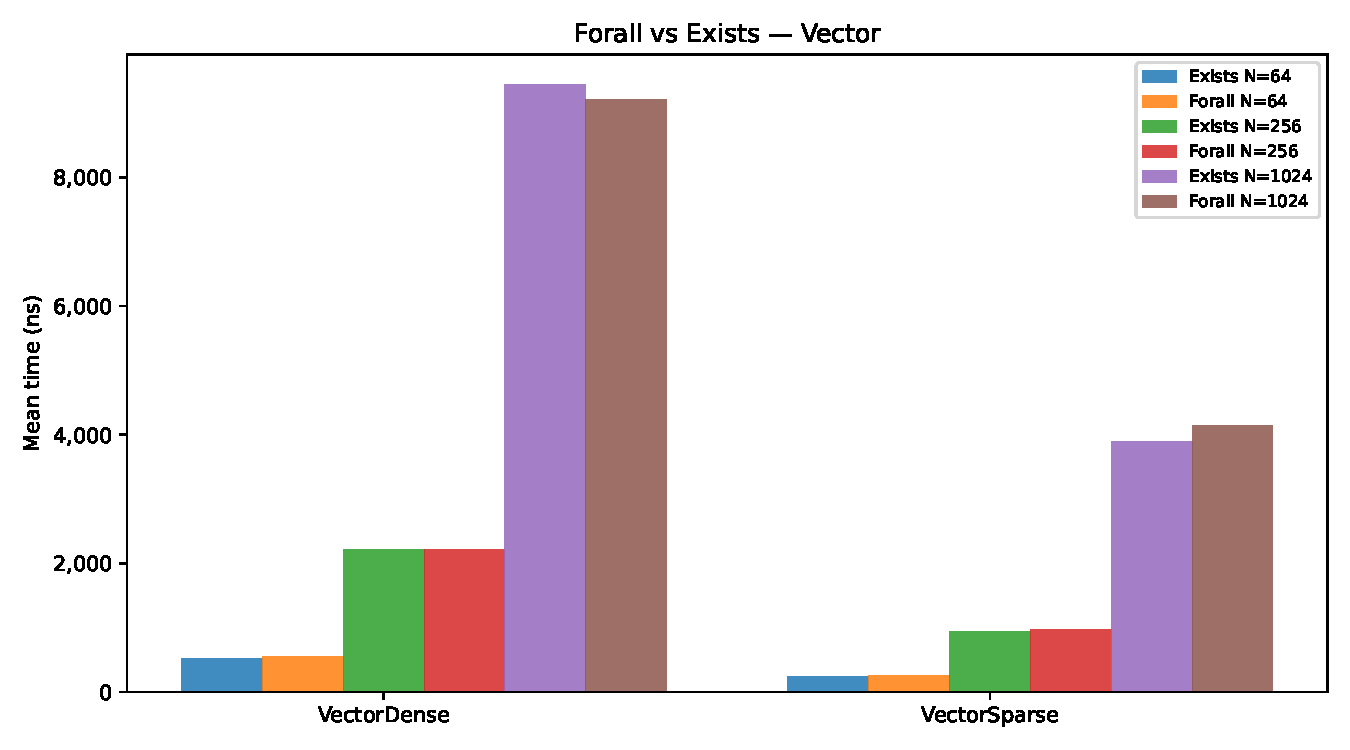
\includegraphics[width=0.92\textwidth]{images/forall_vs_exists_vector.pdf}
\caption{Сравнение exists/forall на векторах}
\label{fig:forall_vect}
\end{figure}

\begin{figure}[H]
\centering
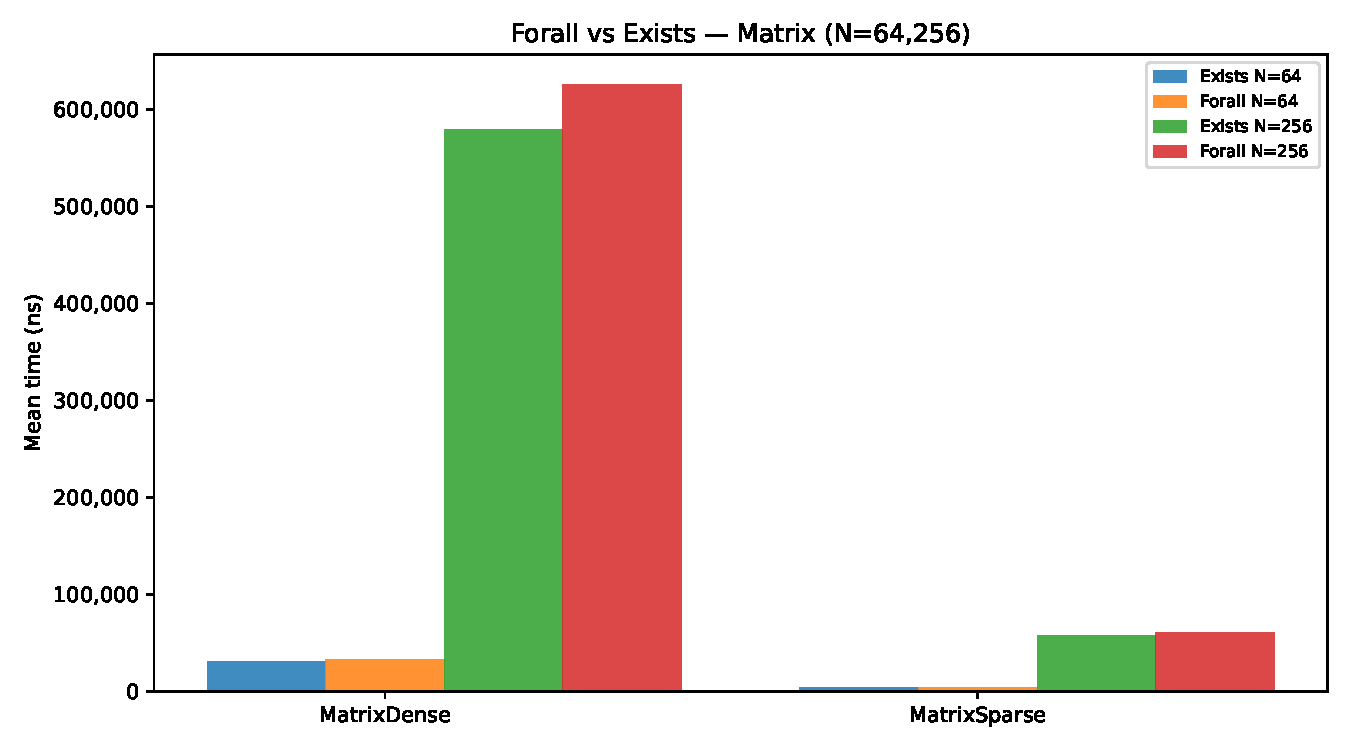
\includegraphics[width=0.92\textwidth]{images/forall_vs_exists_matrix.pdf}
\caption{Сравнение exists/forall на матрицах (N=64, 256)}
\label{fig:forall_mat}
\end{figure}

\begin{figure}[H]
\centering
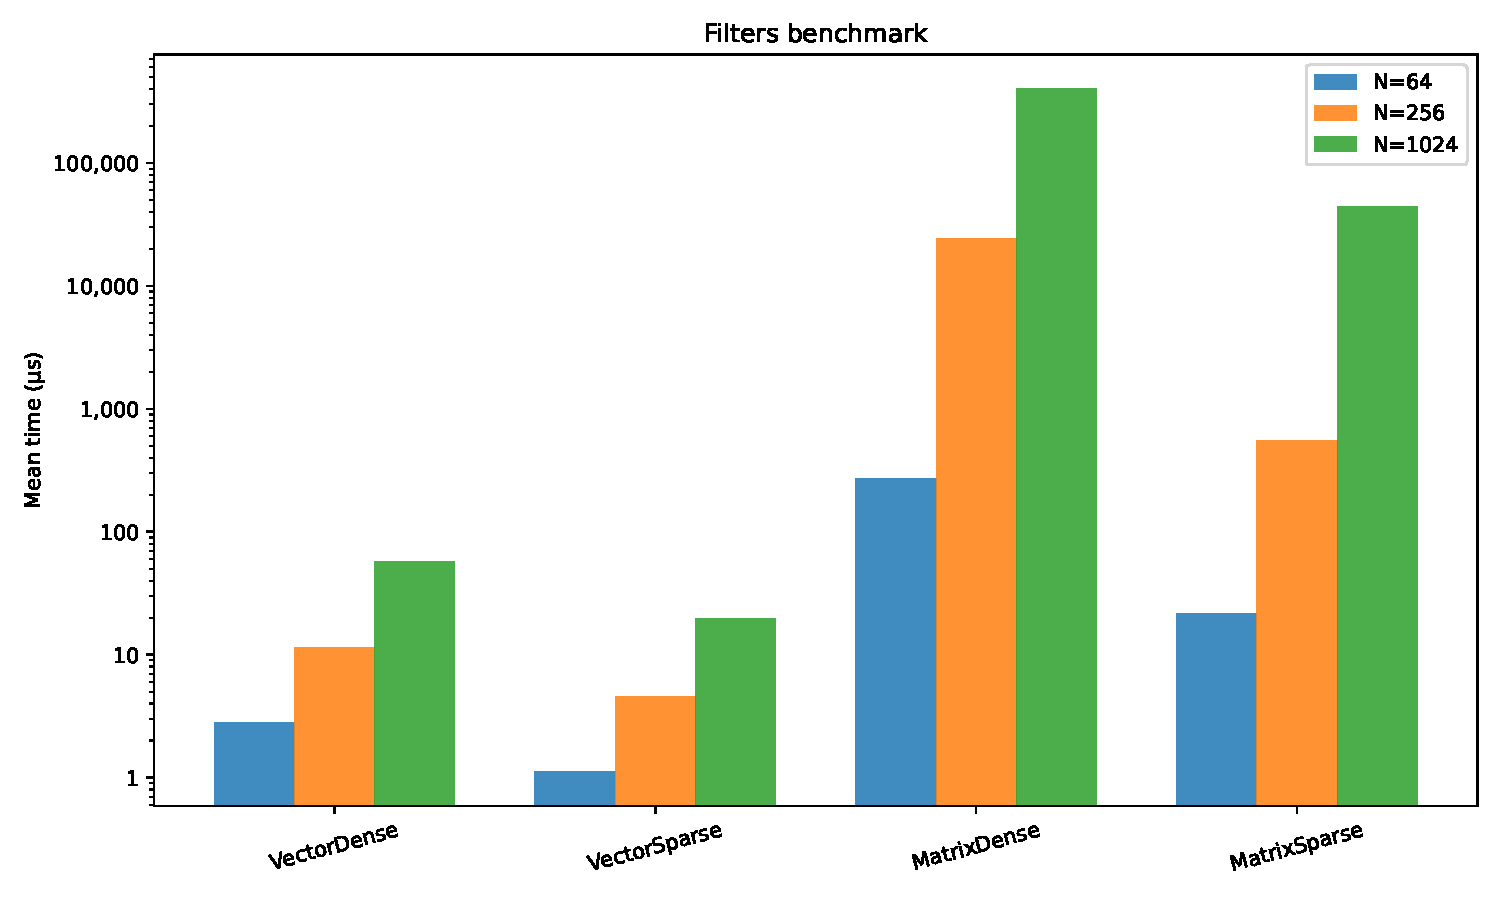
\includegraphics[width=0.92\textwidth]{images/filters_combined.pdf}
\caption{Производительность filter на различных размерах и типах данных}
\label{fig:filters}
\end{figure}

Результаты \texttt{exists} и \texttt{forall} практически совпадают: при выбранных условиях short-circuit не срабатывает (худший случай), поэтому время соответствует $O(N^2)$ на плотных матрицах и $O(N+nnz)$ на разрежённых. В лучшем случае (первый же элемент удовлетворяет \texttt{exists} или не удовлетворяет \texttt{forall}) сложность составит $O(1)$. Выигрыш разрежённого представления (до 3× для векторов, до 15× для матриц) согласуется с отношением числа узлов полного дерева к числу занятых листьев.

\section{Заключение}

В ходе выполнения работы получены следующие результаты:

\begin{itemize}
    \item Реализованы операции \texttt{filter}, \texttt{exists} и \texttt{forall} для разрежённых векторов и матриц на основе деревьев квадрантов.
    \item В \texttt{exists} и \texttt{forall} внедрено короткое замыкание, позволяющее завершать обход досрочно.
    \item Написаны 64 модульных теста для проверки корректности реализованных функций.
    \item Бенчмарки подтвердили ожидаемую асимптотику: $O(N)$ для векторов, $O(N^2)$ для плотных матриц, $O(N+nnz)$ для разрежённых~--- выигрыш до $15\times$.
\end{itemize}

\begin{thebibliography}{99}
\bibitem{qtreefsharp} Репозиторий QTreeFSharp. URL: \url{https://github.com/Lamagraph/QTreeFSharp}
\bibitem{benchmarkdotnet} BenchmarkDotNet. URL: \url{https://benchmarkdotnet.org/}
\bibitem{fsharpdocs} F Sharp Programming. URL: \url{https://en.wikibooks.org/wiki/F_Sharp_Programming}
\bibitem{matplotlib} Matplotlib documentation. URL: \url{https://matplotlib.org/stable/contents.html}
\end{thebibliography}

\section{Репозиторий}
\url{https://github.com/narysh/QTreeFSharp}

\end{document}
